%%%%%%%%%%%%%%%%%%%%%%% file final.tex %%%%%%%%%%%%%%%%%%%%%%
%
% Archivo fuente para el proeycto de trabajo de fin de carrera
%
%%%%%%%%%%%%%%%%%%%%%%%%%%%%%%%%%%%%%%%%%%%%%%%%%%%%%%%%%%%%%%%%%%%

 
\documentclass[spanish,11pt,final]{book}

\usepackage[T1]{fontenc}        % Codificación de fuentes
\usepackage[utf8]{inputenc}     % Codificación para caracteres especiales
\usepackage{ae,aecompl}         % Usar fuentes vectoriales
\usepackage[spanish]{babel}     % Nombres en español
\usepackage{hyperref}           % Hiperenlaces en PDF
%\usepackage{palatino}
\usepackage{bookman}
%\usepackage{gfsartemisia}

\usepackage{listings}		% Listados de código


\usepackage{xspace}
%\usepackage{epsfig}
\usepackage{verbatim}
\usepackage{moreverb}
\usepackage{multicol}
\usepackage{amsmath}
\usepackage{eurosym}
\usepackage{subfigure}
\usepackage{multirow}
\usepackage{fancyhdr}
\usepackage{makeidx}
\usepackage{rotating}
\usepackage{supertabular}
\usepackage{hhline}
\usepackage{array}
\usepackage{cite}
\usepackage{wrapfig}
\usepackage{longtable}
\usepackage{afterpage}



%se utiliza para numerar las \subsubsection
\setcounter{secnumdepth}{5}

%para hacer que las \subsubsection aparezcan en el indice
\setcounter{tocdepth}{5}

% Ruta de las imagenes
\graphicspath{{img/}}


% Definición de entornos nuevos

\newenvironment{narrow}[2]{%
\begin{list}{}{%
\setlength{\topsep}{0pt}%
\setlength{\leftmargin}{#1}%
\setlength{\rightmargin}{#2}%
\setlength{\listparindent}{\parindent}%
\setlength{\itemindent}{\parindent}%
\setlength{\parsep}{\parskip}}%
\item[]}{\end{list}}

\newenvironment{Lista}
{\begin{list}{}{\setlength{\leftmargin}{0pt}%
\setlength{\parsep}{0pt}%
\setlength{\rightmargin}{0pt}%
\setlength{\topsep}{2pt}}
\item \small{}
}
{\end{list}}

% Incluir código fuente
\newenvironment{codigo}[2]
{
\def\codecap{#1}%
\def\coderefer{#2}%
\begin{table}\begin{center}
}
{
  \end{center}
  \caption{\codecap}
  \label{tab:\coderefer}
\end{table}
}




% Definición de comandos nuevos
\newcommand{\eg}{e.g.,\xspace}
\newcommand{\ie}{i.e.,\xspace}
\newcommand{\etc}{etc.\@\xspace}
%\newcommand{\I}{\index}
\newcommand{\n}{\textbf}
\newcommand{\s}{\small}

\newcommand{\clearemptydoublepage}{\newpage{\pagestyle{empty}\cleardoublepage}}

% Figuras de comparativa
\newcommand{\fig}[2]{
  \begin{figure}[t!]
    \begin{narrow}{-1cm}{-1cm}
      \centering
      \includegraphics[width=\linewidth]{#1}
      \caption{#2}
      \label{fig:#1}
    \end{narrow}
  \end{figure}
}


% Redefinición de comandos
\renewcommand{\theenumi}{\arabic{enumi}}
\renewcommand{\theenumii}{\alph{enumii}}
\renewcommand{\theenumiii}{\roman{enumiii}}
\renewcommand{\tablename}{Tabla}
\renewcommand{\listtablename}{Índice de tablas}
\renewcommand{\c}{\emph}

\renewcommand{\chaptermark}[1]{\markboth{#1}{}}
\renewcommand{\sectionmark}[1]{\markright{\thesection. #1}}

%\voffset=-25pt
%\textheight=630pt
%\textwidth=430pt
\voffset=-2.7cm
%\hoffset=-0.5cm
\textheight=24cm
%\textwidth=17cm
\textwidth=16cm
\oddsidemargin=0pt
\evensidemargin=0pt
\pagestyle{fancy}

\lhead[\fancyplain{}{\bfseries\thepage}]{\fancyplain{}{\bfseries\rightmark}}
\rhead[\fancyplain{}{\bfseries\leftmark}]{\fancyplain{}{\bfseries\thepage}}
\cfoot{}

\makeatletter
\newcommand{\noapp}{\def\@chapapp{\chaptername}
  \renewcommand \thechapter{\arabic{chapter}}
}
\makeatother

%para generar el indice
\makeindex

\usepackage{listings}
\usepackage{longtable}
\usepackage{afterpage}


% Clase del documento.
%\documentclass[runningheads,a4paper,spanish]{llncs}

% Paquetes
%\usepackage[utf8]{inputenc}
%\usepackage[spanish]{babel}
%\usepackage{url}
%\usepackage{graphicx}
%\usepackage{rotating}
%\usepackage{calc}

\newenvironment{narrow}[2]{%
\begin{list}{}{%
\setlength{\topsep}{0pt}%
\setlength{\leftmargin}{#1}%
\setlength{\rightmargin}{#2}%
\setlength{\listparindent}{\parindent}%
\setlength{\itemindent}{\parindent}%
\setlength{\parsep}{\parskip}}%
\item[]}{\end{list}}




%se utiliza para numerar las \subsubsection
\setcounter{secnumdepth}{5}

%para hacer que las \subsubsection aparezcan en el indice
\setcounter{tocdepth}{5}

\begin{document}

\renewcommand{\tablename}{Tabla}
\renewcommand{\listtablename}{Índice de tablas}

\thispagestyle{empty}
\large
\vspace{3cm}
\begin{center}

{
\Large\textbf{UNIVERSIDAD DE ALCALÁ}}  \\
\vspace{1cm}
%nombre de la Escuela (comentar con % en cada caso)
%\textbf{Escuela Politécnica Superior}\\
\textbf{Escuela Técnica Superior de Ingeniería Informática}\\

\vspace{1cm}
%titulaci�n a la que se opta
{\Large\textbf{INGENIERÍA INFORMÁTICA}}\\
\vspace{15mm}
% 
\epsfig{file=logo_uah.eps, height=6cm}
\vspace{1cm}

\textbf{Trabajo Fin de Carrera}\\
\vspace{2cm}   

{\LARGE \textbf{Implantación de un Museo Virtual en el Real Observatorio de Madrid}}

\end{center}
\vspace{4cm}
\begin{flushright}
  Héctor Navarro Martín\\
  2010
\end{flushright}

\newpage
\clearemptydoublepage
\thispagestyle{empty}
\large
\begin{center}
{\Large\textbf{UNIVERSIDAD DE ALCALÁ}}  \\
\vspace{7mm}

%nombre de la Escuela (comentar con % en cada caso)
\textbf{Escuela Técnica Superior de Ingeniería Informática}\\

\vspace{7mm}
{\Large\textbf{INGENIERÍA INFORMÁTICA}}\\
\vspace{2cm}
\textbf{Trabajo Fin de Carrera}\\
\vspace{2cm}   

{\Large \textbf{Implantación de un Museo Virtual en el Real Observatorio de Madrid}}

\end{center}
\vspace{2cm}
\noindent
\begin{tabular}{p{5cm}l}
&Alumno: Héctor Navarro Martín\\
&\\
&Director: José Javier Martínez Herráiz
\end{tabular}

\vspace{1cm}
\begin{center}
  \begin{tabular}{rll}
    \textbf{Tribunal:} & &\\ \\ \\
    &&\\
    & \textbf{Presidente:} \\ \\ \\
    \\
    &&\\
    & \textbf{Vocal 1º:}& \\ \\ \\
    \\
    &&\\
    & \textbf{Vocal 2º:}& 
  \end{tabular}
\end{center}


\vspace{15mm}
\begin{tabular}{p{3cm}c}
  &Calificación: ..........................................................................\\ \\
  &Fecha: ...................................................................................
\end{tabular}

\normalsize

%\clearemptydoublepage
%\thispagestyle{empty}
%\vspace*{4cm}
%\begin{flushright}
%  Agradecimiento1.
%\end{flushright}




\clearemptydoublepage
\chapter*{Agradecimientos}

\begin{flushright}
  \vspace{10mm}
  \emph{A HBO, AMC y ABC, por hacerme más ameno el trabajo.}\hspace{1cm}\\
\end{flushright}


\clearemptydoublepage

\tableofcontents
\listoffigures
\listoftables
\setlength{\parskip}{2mm}

\newpage
\newpage

\clearemptydoublepage
\chapter{Resumen}
\newpage
\clearemptydoublepage
\section{Resumen}

\par El objetivo principal de este proyecto es la implantación de una solución software que desempeñe funciones de museo virtual para el Real Observatorio de Madrid. Además, comprenderá una plataforma de gestión de contenidos operable por personal no informático.
Para ello, la solución propuesta es la búsqueda comparada, elección e integración de una plataforma de gestión de contenidos (CMS), añadiendo, si se da el caso, las funcionalidades no incluidas en el paquete escogido pero sí en los requisitos recogidos de la empresa.
Se hace especial hincapié en la reducción del mantenimiento posterior, la accesibilidad móvil, la facilidad de uso para personal no técnico y la posibilidad de modificar y/o añadir funcionalidades en un futuro.

\par Palabras clave: cms, museo virtual, móvil, wiki
\clearemptydoublepage

\chapter{Memoria}
\newpage
\clearemptydoublepage
\section{Introducción}
El trabajo expuesto en este documento tiene como fin la implantación de un museo virtual en el Observatorio de Madrid. La parte más importante en este tipo de proyectos (y, por extensión, de todos) es la recogida de requisitos y el análisis (en este caso, elección principalmente).
Para poder entender mejor lo que se solicita por parte del cliente es necesario conocer el concepto de ``museo virtual'' al que tratamos de acercarnos. Se trataría de una plataforma accesible físicamente desde puestos instalados en una sala de exposiciones dentro del propio observatorio, accesible en línea desde Internet y que comprenda una base de datos posiblemente reutilizable en el futuro. Con estas pinceladas he deducido que la solución existente (no hay que olvidar que esto es ingeniería) más cercana a lo que se nos pide pasaría, en mi opinión, por un gestor de contenidos o CMS (Content Management System).
Dada la amplísima oferta que hay de estos productos en el mercado, creo conveniente hacer una selección a partir de criterios, unos surgidos y otros sugeridos, analizados mano a mano con el cliente.
A partir de ahí, se escogerá el CMS candidato con mejores cualidades en cuanto a facilidad de uso, bajo mantenimiento y características incluidas por defecto. Las características no comprendidas en esta selección (pero necesarias igualmente) serán incorporadas junto con las diferentes modificaciones previstas para darle forma final a la plataforma. Posteriormente, se integrará y se pondrá en servicio con los plazos que el cliente disponga para ello.

\section{Base teórica}
Al tratarse de un proyecto tan práctico, la base teórica del mismo no tiene un gran misterio. Se trata de realizar el clásico enfoque de presentar distintas aplicaciones al cliente cumpliendo unos requerimientos mínimos y adpatanto e integrando la solución escogida para que encaje con el sistema solicitado.

En esta ocasión, presentaremos varios subapartados según las distintas fases del proyecto.

\subsection{Estado del Arte}
\par Para elaborar este proyecto pensé que lo más sensato era, una vez acotado el problema, tratar de echar un vistazo a cómo estaban las cosas en la actualidad en otros museos. Considero importante saber en qué estado se encuentran tanto el círculo de los CMS, wikis, museos y catálogos informatizados.
En este periplo, he topado con varias fuentes de información desconocidas para mí, algunas ideas sacadas de museos visitados en persona y una exhaustiva (aunque difícil de discernir) cantidad de datos sobre gestores de contenido.

\subsubsection{¿Qué puede ser un museo virtual?}
\par Al hablar de museos virtuales, a uno se le pueden venir a la mente distintos conceptos sobre lo que representan esas palabras:

\begin{itemize}
\item Visita virtual al museo (modo ``Second Life").
\item Galería de imágenes.
\item Sitio web del museo (meramente informativo).
\item Catálogo de objetos.
\item Ampliación de lo expuesto en el museo.
\end{itemize}

\par En el primer caso, nos referimos a esa idea de recrear a través de gráficos en 3D la experiencia de una visita real al museo. Esta solución es muy poco usada debido a lo costoso de la misma. Además de modelar infográficamente la arquitectura del museo y construir una aplicación que utilice un potente motor gráfico para sostenerla, hay que tener en cuenta el gran tráfico generado para que esto funcione adecuadamente. En mi opinión, dado que difícilmente se puede reemplazar la experiencia de visitar el museo en persona, creo que no compensa tanto despliegue de medios ya que no contribuye (al menos en el caso expuesto) sensiblemente al objetivo marcado.

\par El segundo caso, una mera galería de imágenes, aunque pobre, podría vale como museo virtual para un museo de arte en según qué circunstancias. Obviamente, y aunque la presentación de la información en este formato sea algo a tener en cuenta, si limitáramos nuestro museo virtual a este tipo de sitio, estaríamos, creo yo, limitando muchísimo la información ofrecida, cosa que no cuadra con el objetivo de complementar el museo.

\par El tercer caso lo he incluído como posibilidad de que alguien lo identificase al hablar de ``museos virtuales", dado que crear una página con información corporativa, de horarios y accesos es sólo una parte de lo que pretendería este proyecto.

\par El cuarto caso será aquel en el que básicamente tenemos una somera base de datos con una sencilla interfaz de búsqueda y acceso a la colección, sin tratar de explicar o poner en contexto los objetos que tenemos delante.

\par El quinto caso es el que nos ocupa, siendo el cometido del mismo complementar la exposición física, permitiendo a los visitantes (y no visitantes) conseguir un trasfondo y una explicación más completa de los objetos y su contexto para contribuir a la divulgación de un conocimiento relacionado con lo expuesto. Obviamente incluirá parte de galería de imágenes en cuanto a interfaz, información de típico sitio web como caso anecdótico de contenido, componentes que mejoren la interactividad sin sacrificar el desempeño y el coste y datos concretos sobre los objetos como manera de acceder a la base de datos. 

\subsubsection{Museos}

\par Aprendiendo de museos conocidos, podemos poner ejemplos prácticos de los que sacar ideas o matices que el cliente pueda identificar como deseables. Está claro que sería imposible abarcar todos o siquiera la mayoría de los museos del mundo, ni siquiera los más importantes (¿quién decide esa lista?), pero sin embargo sí se pueden incluir ideas que hayamos rescatado de otras implementaciones satisfactorias.
Algunos ejemplos son:

\paragraph{Tate Modern (Londres, Reino Unido)}
\par Pude comprobar en directo algunas de las ideas puestas en práctica por esta entidad gracias a un viaje reciente. Allí pude ver buenas ideas como el acercamiento de los contenidos de las salas al gran público (en especial, a niños) a base de actividades interactivas que introducían con naturalidad y entretenimiento conceptos difíciles de asimilar de otra manera. Sin duda es una buena idea, aunque no se encuadra en este proyecto, podría ser considerada para futuros trabajos. 
\par Más concretamente, en materia de museos virtuales, vi la adopción de terminales de mano que complementan la experiencia del visitante físico. Estamos acostumbrados a ver las típicas guías locutadas en diversos idiomas que nos amplían el contenido de las exposiciones introduciendo un número del índice de grabaciones. Suelen ser aparatos con usos muy restringidos (especiales para museos) con lo que eso supone para el coste final para el museo. En cambio, en este caso, se trataba de dispositivos móviles que están en el mercado, en nuestro caso, una especie de PDA de marca Toshiba o Dell (según renovaciones). Son dispositivos básicos que permiten mostrar contenidos web y multimedia sin muchas complicaciones. Esto es: pantalla en color, interfaz intuitiva, salida de auriculares y conectividad inalámbrica. Este último punto permite renovar sin coste temporal importante (y de manera transparente al visitante) los contenidos presentados. El hecho de que sea un dispositivo común abarataría los costes, premitiendo, incluso, trabajar con tecnología no necesariamente de última generación, dada la baja exigencia de los contenidos a presentar. Parece evidente que será más fácil conseguir un buen precio por una buena cantidad de dispositivos a punto de ser retirados del mercado o símplemente de stock sobrante.
Debajo de todo esto subyace la idea de utilizar unos estándares mínimos, aunque sean estándares de facto. Esto nos permitiría (como en el caso del Tate Modern) reemplazar los dispositivos por otros nuevos sin hacer cambios significativos en la plataforma y haciendo que coexistiesen ambos modelos. Y lo que es, quizá, más interesante, dar la opción a usuarios que posean dispositivos con capacidades similares a los ofrecidos de conectarse al museo virtual por su cuenta y en directo, ahorrando bastante en costes.

\begin{figure}
\begin{narrow}{-0.1\linewidth}{-0.1\linewidth}
\centering
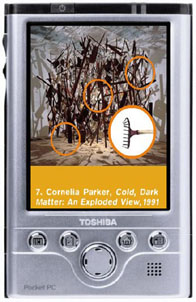
\includegraphics{tatehandheld}
\caption{Imagen de dispositivo de mano del Tate Modern\cite{references:tatehandheld}}
\end{narrow}
\label{fig:moma}
\end{figure}



\paragraph{MoMA (New York, EEUU)}
\par Este apartado, desgraciadamente, se refiere a las ideas y modelos observados directamente en su página web. Nos encontramos con ideas, sobre todo en cuanto a presentación visual de contenidos. Digamos que la idea de presentar los contenidos en una matriz de imágenes con pies identificativos que, al pulsar sobre ellas, nos lleven a la información específica de ese objeto podría ser cercana a lo buscado. También sería una idea a tener en cuenta la categorización de las obras por área temática, época o tipo de objeto, aunque no lo firmamos como algo seguro en nuestra plataforma. Por último, reseñar que ellos parece que hacen (o al menos tienen la posibilidad de hacer) uso de la vista ``por perspectivas". Esto sería como tener una lista desplegable en la pantalla que nos permitiera fácilmente cambiar entre los distintos puntos de vista (como si de idiomas se tratara) pudiendo adaptar la plataforma a una presentación para , por ejemplo, niños, estudiantes o expertos en el tema. El sistema finalmente escogido para implementar esa ``granularidad'' de contenidos se tomó de otro sitio web que veremos más adelante.

\begin{figure}
\begin{narrow}{-0.1\linewidth}{-0.1\linewidth}
\centering
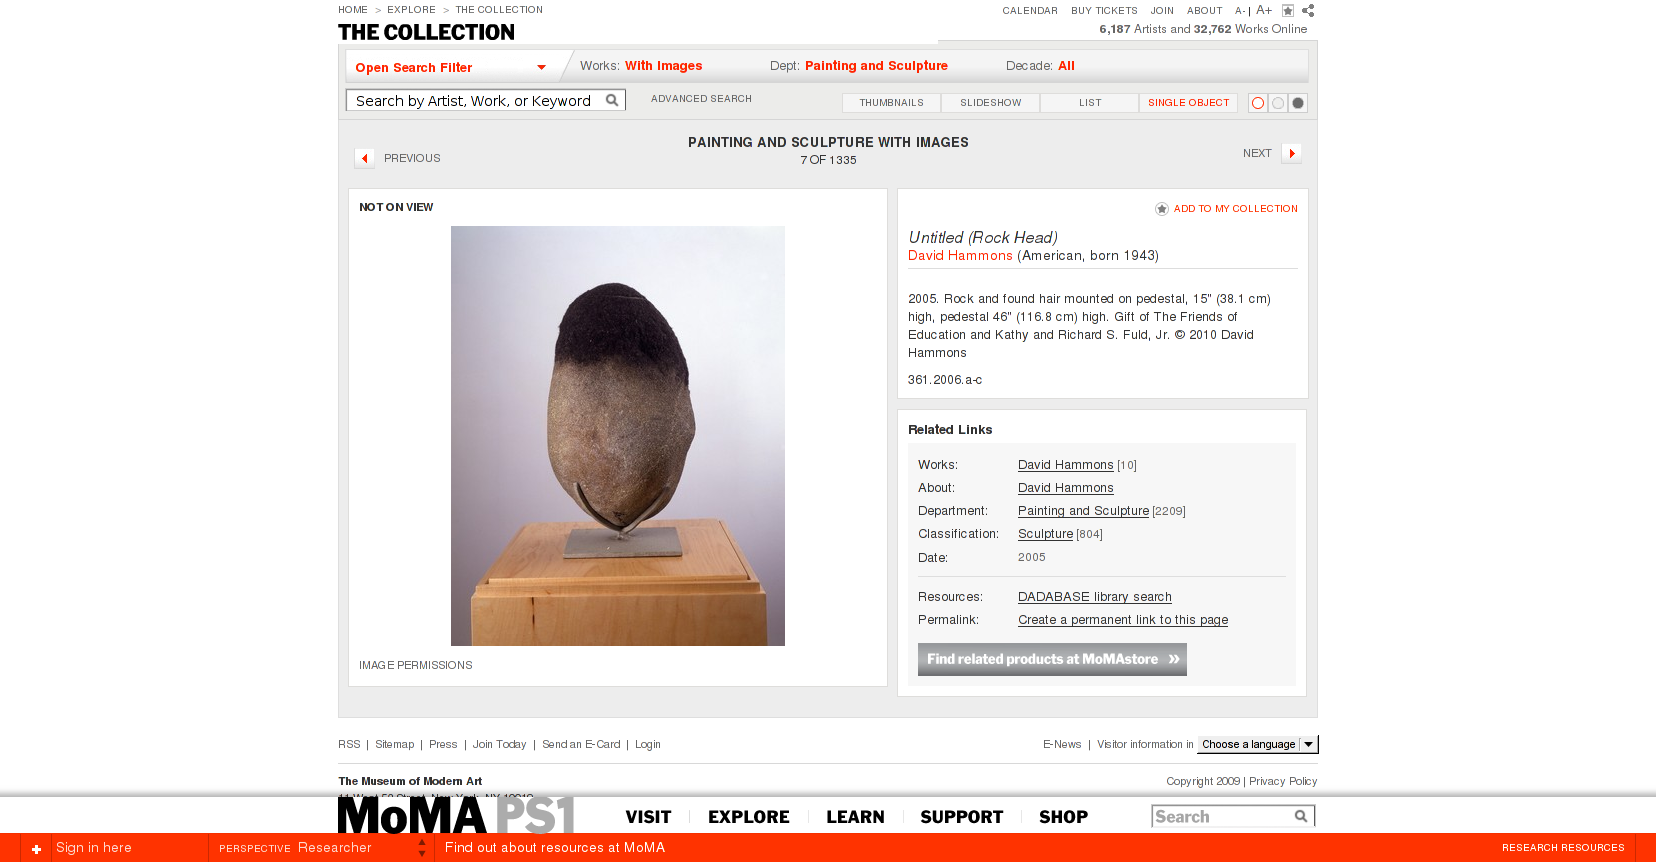
\includegraphics[width=\linewidth]{capturamoma}
\caption{Captura de pantalla del sitio del MoMA}
\end{narrow}
\label{fig:moma}
\end{figure}



\paragraph{Actual museo del OAN}
\par Existe una versión antigua del museo virtual del Observatorio Astronómico Nacional, cuya información será contenida presumiblemente cuando se complete el contenido de la plataforma objeto de este proyecto. Si entramos al sitio web que lo hospeda dentro del sitio del Instituto Geográfico Nacional (Ministerio de fomento) descubrimos una estructura de navegación con algunas deficiencias para movernos entre objetos, para dar un vistazo rápido y desde luego una descontextualización importante. Podríamos catalogarlo como uno de esos museos virtuales del caso cuarto, un catálogo de objetos. No se puede negar su utilidad pero son las funciones de las que carece las que hacen necesaria la creación del proyecto actual.

\begin{figure}
\begin{narrow}{-0.1\linewidth}{-0.1\linewidth}
\centering
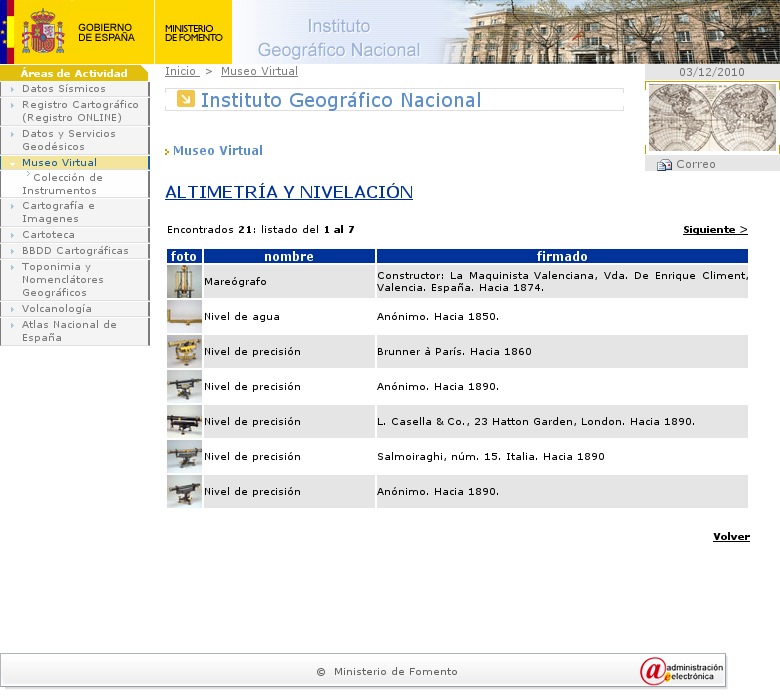
\includegraphics[width=\linewidth]{capturamvoan}
\caption{Captura de pantalla del museo virtual del OAN}
\end{narrow}
\label{fig:oan}
\end{figure}

\subsubsection{Enciclopedias}

\par Como parte de la gestión del conocimiento, además de las webs de los propios museos, he indagado en otras webs que se dedican a funciones parecidas (no olvidemos que el museo al que se refiere este trabajo dista de ser un museo de arte) a lo que queremos conseguir en cuanto a organización del conocimiento.

\paragraph{Wikipedia}
\par Digamos que este sería el paradigma de enciclopedia dinámica y colaborativa hoy en día. Es más o menos familiar para cualquier persona que use con asiduidad internet (sobre todo para buscar información) y aunque sus fuentes, consistencia y fiabilidad puedan ser cuestionables, su manera de disponer la información no puede tomarse en absoluto como mala. De aquí podríamos tomar en consideración el aspecto colaborativo del medio, pero en reuniones con el cliente se convino que al ser una institución de referencia, los contenidos (aunque aportados por diferentes personas) debían ser acotados a unos poco usuarios (generalmente trabajadores) y moderados en última instancia por la figura de un editor que revisaría y daría el visto bueno a los mismos.
La disposición de portal inicial ofrecida por este sitio es una idea que podría funcionar en nuestro caso, incluyendo esos pequeños ``ganchos'' que cambian diaria o aleatoriamente para que determinados artículos puedan ser descubiertos por un navegante no asiduo. Además, mantiene una división temática necesaria para el sitio y tiene un sistema de control de versiones válido para documentos escritos, así como la relación semántica de entradas y la inclusión de contenido multimedia fácilmente.
Referido al punto anterior, hay que señalar que, en un principio, se ha optado por la manera de Wikipedia de ampliar la profundidad de un artículo: en vez de diseñar distintas capas para distintos individuos, enlazar los artículos que profundizan sobre un tema para que sea el usuario el que decida cuándo parar.


\paragraph{Indianopedia, Frikipedia, *pedia}
\par Esta entrada engloba varios sitios por una razón: existe un fenómeno creciente que consiste en que cada ``ecosistema'' de conocimiento puede generar su propio repositorio de información. Esto contribuye a diversificar las fuentes evitando fraudes y manipulaciones, a la vez que descentraliza y permite pluralidad de visiones. Igual que existen el diccionario de la RAE, María Moliner, Espasa Calpe, etc., el concepto de la propia enciclopedia, en nuestro caso, puede servir para contener los artículos a los que no llegan otras enciclopedias más generales o de los que tenemos un conocimiento certero y fuentes propias.

\subsubsection{Sistemas gestores de contenidos vs Wikis}
\par Llegados a este punto parece evidente el camino que estamos sugiriendo. Para crear nuestra plataforma y que tenga algunos factores básicos como diferentes presentaciones al usuario (al menos internet y móviles), incluya una base de datos, interfaz amigable para creadores de contenido no informáticos y demás funciones de administrador facilitadas al máximo.

En un principio se tuvo la tentación de basar toda la plataforma en un mero wiki (La base de datos más simple del mundo) pero se vio que las características más destacables de un wiki nos sobraban salvo la facilidad de edición y de uso, que se puede apreciar también en los CMS más comunes. Además, claro está, si nos ciñéramos a un simple wiki estaríamos renunciando a una serie de herramientas útiles que ya se integran en los CMS con naturalidad.

De la toma de decisiones sobre la elección de plataforma base hablaré en la sección de diseño.


\section{Descripción del diseño}

\subsection{Baremación de alternativas}
\par Llegados a este punto, nuestro proyecto tiene que empezar a definirse y descartar unas alternativas de otras. Hasta la fecha, recapitulando, hemos puesto encima de la mesa la necesidad de un gestor de contenidos con o sin componente wiki. A este esqueleto inicial habría que añadirle una serie de características y su grado de importancia (donde 0 es prescindible y 5 es imprescindible). Este grado de importancia ha sido recogido en entrevista directa con responsables de la supervisión del proyecto.

\subsubsection{Relación de características}

\begin{tabular}{l @{\hspace{10px}} r}
Caracerística & Nota \\
\hline \\
Interfaz de creador en español & 4 \\
Interfaz de usuario en múltiples idiomas & 5 \\	
Varias perspectivas diferenciadas & 1 \\
Web semántica & 0 \\
Uso de estándares & 0 \\
Editor WYSIWYG & 5 \\
Soporte comercial & 1 \\
Comunidad de desarrolladores / soporte & 4 \\
Actualizaciones recientes & 1 \\
Entorno colaborativo & 3 \\
Buzón de sugerencia / Preguntas frecuentes & 0 \\
Página de control de cambios / CVS & 5 \\
Licencia libre & 5 \\
Base de datos & 3 \\
Sistema de ficheros (en contraposición a BD) & 0 \\
Posibilidad de exportar a pdf/LaTeX & 1 \\
Versión para plataformas móviles & 4 \\
Blog & 0 \\
\end{tabular}

\subsubsection{Comentarios}

\par La cuestión sobre las perspectivas diferenciadas se ha decidido plantear a la manera de Wikipedia, es decir, a base de enlaces con contenido más exhaustivo en vez de un selector de perspectiva que nos dejase ``ponernos las gafas'' de ``estudiante", ``visitante'' o ``investigador'' con un botón, al menos, en esta fase del proyecto.

\par Aun no habiendo resuelto temas importantes como si la figura del ``responsable de mantenimiento'' de la aplicación existirá y quién se encargaría de ella, en la misma reunión se esbozó la idea de que existiría una fase inicial de carga con un principio y un final y una fase de mantenimiento en la que se harán cambios pero a menor ritmo. Todas ellas irán recubiertas de la figura del supervisor, que se encargará de aprobar o rechazar los cambios u añadidos propuestos por los generadores de contenido antes de que éstos se reflejen en la producción final.

\par En contrapartida a las ideas de blog y buzón de sugerencias, se propondrá (con mayor o menor grado de insistencia) al usuario realizar una encuesta evaluación con su propio espacio para sugerencias.

\par El tema de uso de estándares y web semántica, si bien es un objetivo deseable, no debe obstaculizar el resto de ellos, se asume de la última reunión.

\par Por último, y para que la base de datos creada pueda ser fácilmente usada por otros proyectos, se ha optado por buscar una solución orientada a bases de datos y no a sistemas de ficheros como modo de almacenamiento. Esto descartará unas cuantas opciones.

\subsection{Comparativa}

\par Habiendo descartado o relativizado la importancia de algunos de los requerimientos iniciales para nuestro gestor de contenidos, vamos a tratar de hacer una propuesta inicial. Para ello, vamos a utilizar herramientas gratuitas en línea que presentan los datos como una matriz de características (CMSMatrix.org y CMSMatch.com), aunque sólo se presentan en este documento las relativas a la primera, puesto que la segunda carecía de un montón de datos relevantes.

\subsubsection{Premisas iniciales}
\par Las premisas iniciales para los CMS (y las que más descartan) son:

\begin{itemize}
\item Más populares y mejor puntuados. De esta manera potencialmente hayaremos estabilidad y una comunidad de soporte activa. Para ello, echaremos un vistazo a las estadísticas disponibles en la red sobre CMS más utilzados, mejor puntuados y más premiados, tratando de sopesar adecuadamente cada fuente.
\item Editor visual (WYSIWYG Editor / Drag'n'Drop interface).
\item Con capacidad para gestionar la plataforma en varios idomas (Internationalization = Multilingual Content / Multilingual Content Integration / Web-based Translation Management).
\item Página de cambios (Versioning / Asset Management=Media Library)
\item Coste cero.
\item Licencia OpenSource.
\item Comunidad de desarrolladores (Developer Community).
\item Interfaz en español (Interface Localization).
\item Versión para móviles (Mobile Internet).
\end{itemize}

\subsubsection{Candidatos pre-seleccionados}
\par Primeros elegidos por su demostrada utilización, premios, etc:

\begin{enumerate}
\item dotCMS
\item Drupal
\item Joomla!
\item LifeRay Portal
\item MODx
\item mojoPortal
\item Moodle
\item Plone
\item SilverStripe
\item WordPress
\end{enumerate}

\par El primer problema que encontramos es que estos sistemas que hemos elegido para comparar los diferentes CMS no nos dejan saber qué idiomas tiene la interfaz de usuario, así que ha que hacer una pequeña investigación entrando en las páginas web de cada uno de los sitios. Tras esto, sabremos que, al menos en cuanto a la interfaz de administración, todas las plataformas preseleccionadas pueden ejecutarse en español.


\par A continuación, pasamos a desgranar las secciones más interesantes de la comparativa reseñada:

\subsubsection{Comparativa con CMSMatrix}

\par En esta ocasión, vamos a ir comparando las características más reseñables de cada producto, por bloques, según está organizado en el servicio consultado.

\paragraph{System Requeriments (Requisitos de sistema)}

\par Vamos a ir analizando lo que se ve en la figura:

\begin{figure}
\begin{narrow}{-0.12\linewidth}{-0.12\linewidth}
\centering
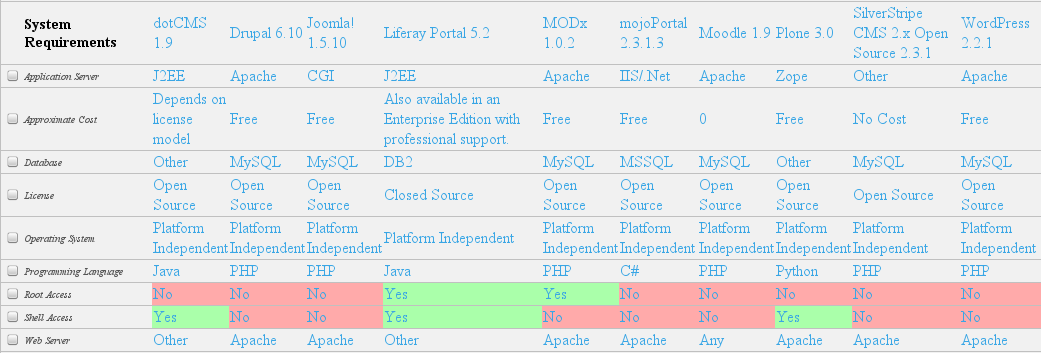
\includegraphics[width=\linewidth]{cmsmat1}
\caption{System Requeriments desde CMSMatrix.org}
\end{narrow}
\label{fig:cmsmat1}
\end{figure}

\par En este caso, debemos fijarnos en la parte ``License'' principalmente, comprobando que todos menos Liferay Portal ostentan una licencia libre. Posteriormente he podido comprobar que la licencia de Liferay Portal cambió de licencia MIT a LGPL a partir de la versión 6\cite{references:liferaylicense}, así que, a falta de argumentación en contra sobre los pormenores de cada licencia, todos entrarían dentro del requisito principal.

\par Hay que comentar que una de las guías sugeridas por la empresa era que, de ser posible, la plataforma fuese familiar con lo que ya se conoce en la casa por parte de los trabajadores fijos. En este caso, las cosas irían si no ya por la plataforma en sí, por el lenguaje de programación el que están programados, siendo estos Java, PHP, Phyton y C Sharp los que ocupan nuestra comparativa.

\paragraph{Security (Seguridad)}

\par Según el gráfico de debajo, los datos que más nos interesan son ``Content Approval'' (aprobar contenidos antes de publicación), ``Granular Privileges'' (posibilidad de tener distintos privilegios para cada usuario o grupo de usuarios), ``Versioning'' (control de versiones).

\par La única opción con inconvenientes en este campo sería Joomla!, que según cmsmatrix no permite la asignación de privilegios personalizada, señalando que MODx en supervisión de contenidos y control de versiones necesitaría un añadido gratuito, al igual que Joomla! para este último caso.

\begin{figure}
\begin{narrow}{-0.12\linewidth}{-0.12\linewidth}
\centering
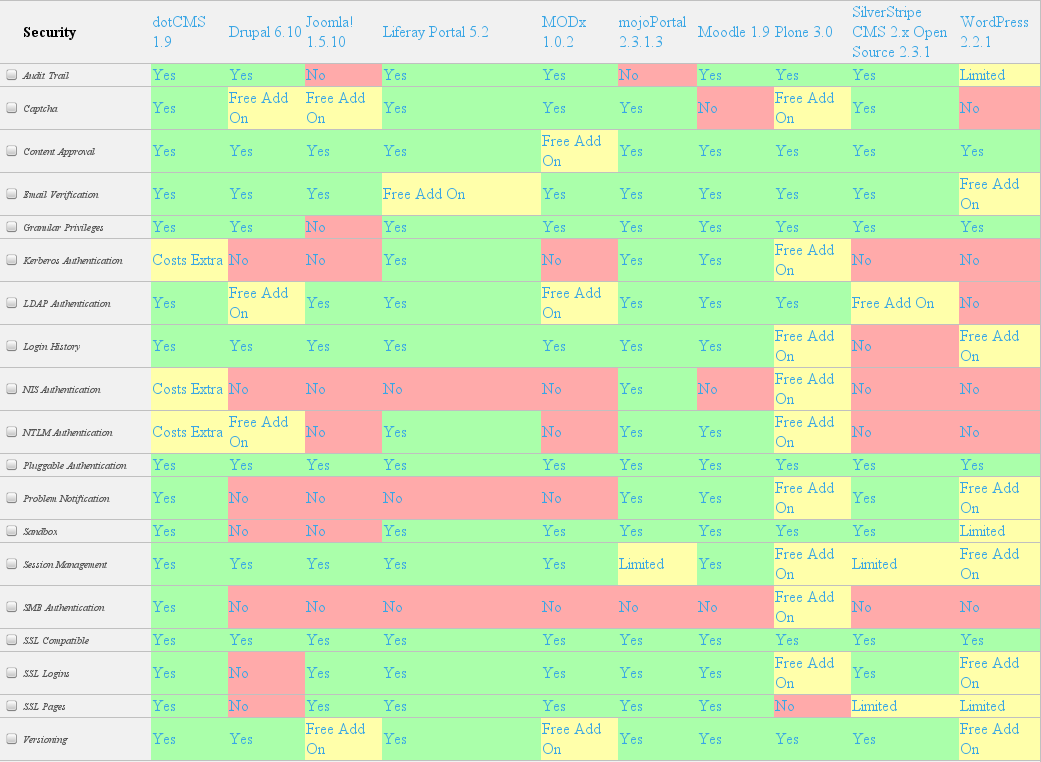
\includegraphics[width=\linewidth]{cmsmat2}
\caption{Security desde CMSMatrix.org}
\end{narrow}
\label{fig:cmsmat2}
\end{figure}

\paragraph{Support (Asistencia)}

\par Esta es una de las partes menos importantes de la comparativa, pues es incierto el futuro en cuestión de mantenimiento de la plataforma. En este caso nos estaríamos fijando más en ``Commercial Support'' (asistencia de pago), ``Developer Community'' (comunidad de desarrolladores) y ``Public Forum'' (foros públicos). Destacar únicamente que WordPress no dispone de ese servicio, aunque el servicio gratuito sí que exista.

\begin{figure}
\begin{narrow}{-0.12\linewidth}{-0.12\linewidth}
\centering
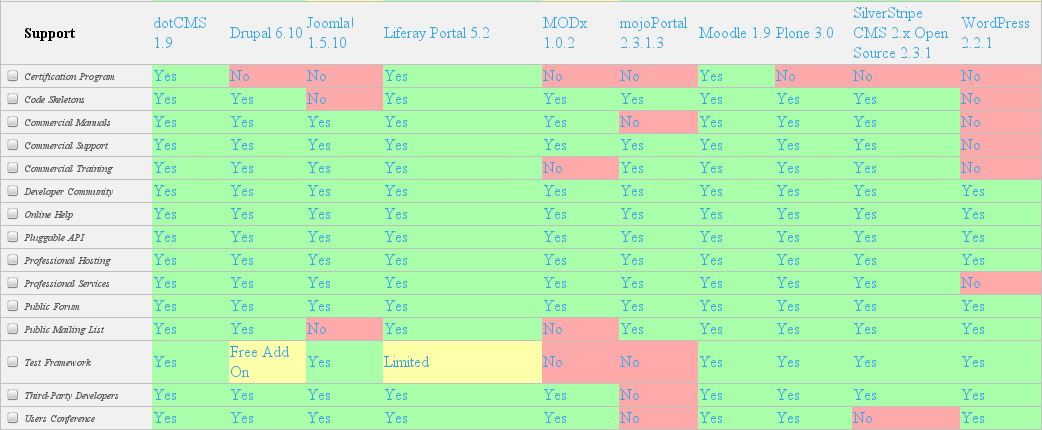
\includegraphics[width=\linewidth]{cmsmat3}
\caption{Support desde CMSMatrix.org}
\end{narrow}
\label{fig:cmsmat3}
\end{figure}

\paragraph{Ease of Use (Facilidad de uso)}

\par Este es uno de los puntos más importantes de la comparativa. Si observamos:

\begin{figure}
\begin{narrow}{-0.12\linewidth}{-0.12\linewidth}
\centering
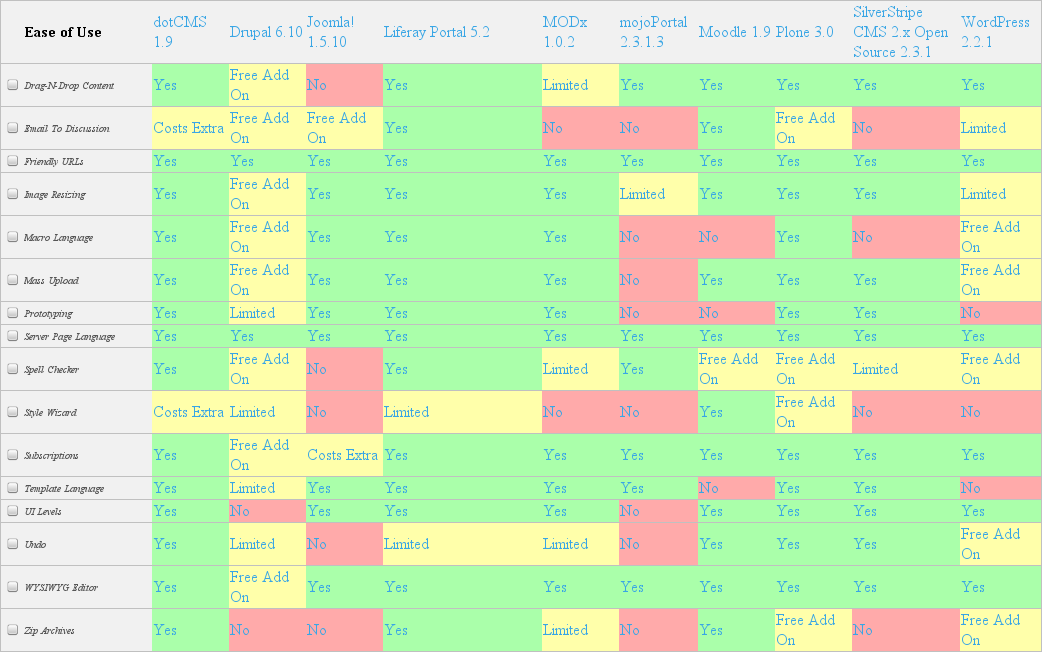
\includegraphics[width=\linewidth]{cmsmat4}
\caption{Ease of Use desde CMSMatrix.org}
\end{narrow}
\label{fig:cmsmat4}
\end{figure}

\par Encontraremos que, a destacar, podemos seleccionar como las más relevantes las opciones de ``Drag-N-Drop Content'' (arrastrar y soltar contenido), ``Image Resizing'' (redimensionado de imágenes), ``Mass Upload'' (subida de archivos masiva) y ``WYSIWYG Editor'' (editor visual).
\par De la primera característica, tenemos Joomla! que no la soporta, MODx con una implementación limitada y ``Drupal'' con un añadido para esa función. De la segunda, tendríamos que tanto ``mojoPortal'' como ``WordPress'' presentan esta función limitada y ``Drupal'' necesita, otra vez, añadidos. En cuanto a la subida de ficheros masiva, mojoPortal sería incapaz mientras que Drupal y WordPress necesitarían un add-on. El editor visual está presente en todas, aunque se nos avisa que Drupal necesita de un añadido también. Lo que nos hace pensar que Drupal está construido de forma modular ya que muchas de sus características se consiguen a través de módulos suplementarios. Esto puede tener consecuencias positivas en cuanto a agilidad, tamaño y complejidad y negativas en cuanto que el proceso inicial de puesta en marcha puede (aún no lo sabemos) ser más complicado que otros.



\paragraph{Performance (Rendimiento)}

\par Este apartado no contiene aspectos demasiado relevantes para el proyecto que tenemos entre manos, pues no se espera que la carga de trabajo del servidor sea elevada como para preocuparse por estos detalles, aunque llegado el momento del desempate, podría declinar la balanza entre una opción y otra. Siendo tanto ``WordPress'' como ``Joomla!'' los más perjudicados.

\begin{figure}
\begin{narrow}{-0.12\linewidth}{-0.12\linewidth}
\centering
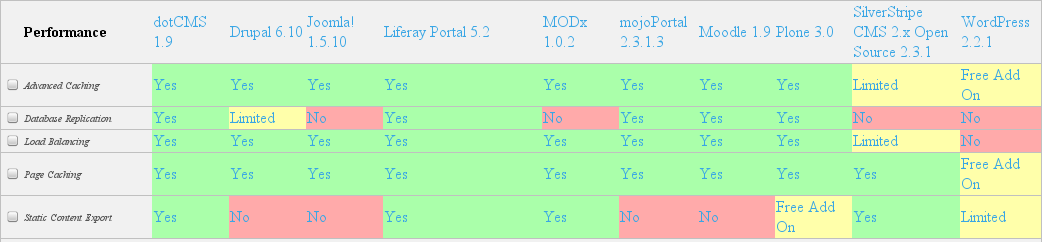
\includegraphics[width=\linewidth]{cmsmat5}
\caption{Performance desde CMSMatrix.org}
\end{narrow}
\label{fig:cmsmat5}
\end{figure}


\paragraph{Management (Administración)}

\par La figura presenta aspectos importantes para el administrador de la plataforma como: ``Online Administration'' (gestión en línea), ``Themes/Skins'' (temas gráficos), ``Web-based Style/Template Management'' (gestión de estilos y plantillas vía web) y ``Web-based Translation Management'' (gestión de traducciones vía web).

\begin{figure}
\begin{narrow}{-0.12\linewidth}{-0.12\linewidth}
\centering
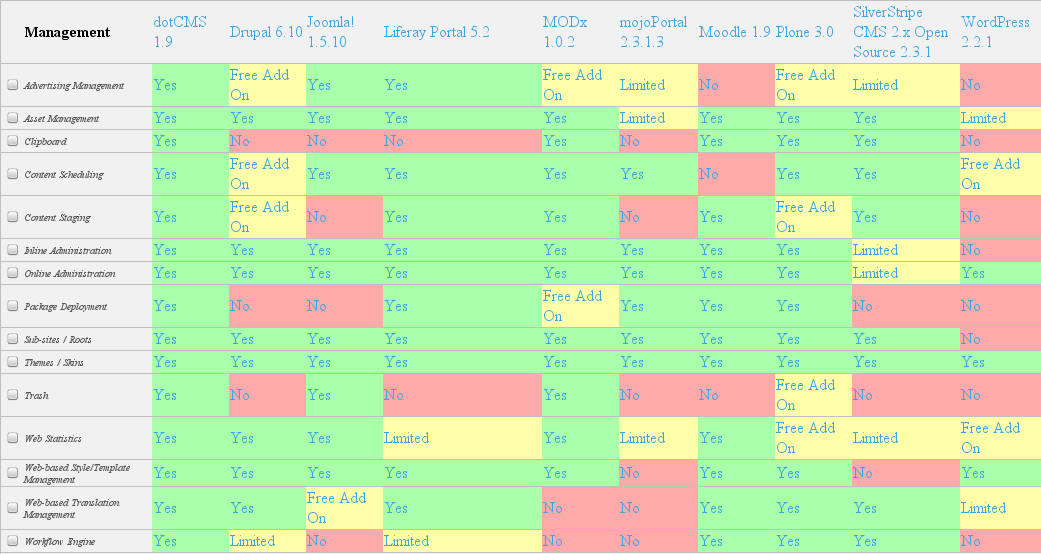
\includegraphics[width=\linewidth]{cmsmat6}
\caption{Management desde CMSMatrix.org}
\end{narrow}
\label{fig:cmsmat6}
\end{figure}

\par Las características que he citado primera y cuarta son, a mi juicio, fundamentales, ya que permiten la gestión de la plataforma virtualmente desde cualquier dispositivo que pueda mostrar páginas web. Las fallas más significativas son las de ``MODx'' y ``mojoPortal", que gracias a la falta de gestor de traducciones vía web quedarían, por ahora, descalificadas por completo. Hay que destacar que ``WordPress'' tiene limitaciones en esto y acumularía ya unas cuantas pegas que no lo hacen muy aconsejable.


\paragraph{Interoperability (Interoperatividad)}
\par Toda las características mostradas en la tabla siguiente tienen una importancia técnica alta, aunque su repercusión en el resultado visual final no sea grande. Quiero, en este apartado, analizarlas una por una para que se sepa de qué trata cada una.

\par Content Syndication (RSS) (sindicación de contenidos): Se trata de un sistema que permite a los usuarios estar al tanto de las nuevas publicaciones de una plataforma. Como en nuestro caso el contenido será mayoritariamente estático no es algo relevante.

\par FTP Support (soporte para transferencia de ficheros por FTP): FTP es un protocolo especialmente diseñado para la transferencia de ficheros, siendo, aunque ahora menos utilizado, un valor más. Su importancia es media.

\par UTF-8 Support (soporte para codificación UTF-8): Esta codifiación es la que pretende ser universal para la inmensa mayoría de idiomas. Utilizarla es un paso adelante para la interoperatividad de aplicaciones, pero no es altamente relevante para el proyecto.

\par WAI Compliant (cumple con WAI): Web Accessibility Initiative (Iniciativa para la Accesibilidad Web) es una serie de reglas que buscan la accesibilidad de los contenidos para usuarios impedidos. Propone unos mínimos y puede ser interesante implementarlo, aunque no vital.

\par WebDAV Support (soporte para WebDAV): ``Edición y versionado distribuidos sobre la web'' es, en esencia, un protocolo que nos permite cambiar a distancia los contenidos de un servidor con cualquier aplicación que lo implemente (sin necesidad de una herramienta propia). No es imprescindible ni es el único modo.

\par XHTML Compliant (cumple con XHTML): XHTML es una especificación que trata de dar coherencia y acercar el lenguaje HTML a los estándares XML. Busca la ausencia de errores (se puede validar con facilidad) y la fiel reproducción de un contenido en distintos navegadores sin demasiadas diferencias. Es decir, busca establecer un estándar. Yo lo consideraría un mínimo exigible para cualquier plataforma web aunque en el futuro se de la posibilidad de cambiar a otros estándares como HTML5 (que aún no están implantados masivamente).


\begin{figure}
\begin{narrow}{-0.12\linewidth}{-0.12\linewidth}
\centering
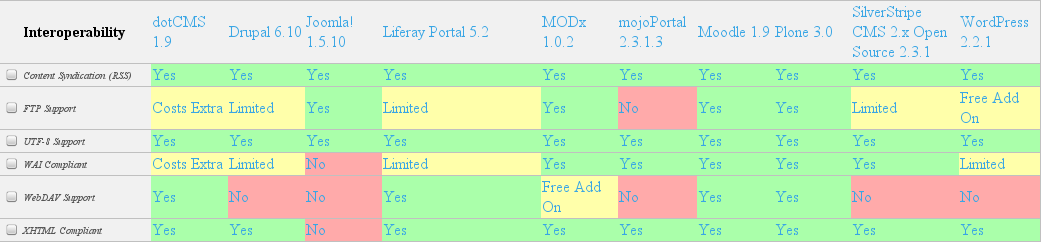
\includegraphics[width=\linewidth]{cmsmat7}
\caption{Interoperability desde CMSMatrix.org}
\end{narrow}
\label{fig:cmsmat7}
\end{figure}



\paragraph{Flexibility (Flexibilidad)}


\par De esta sección, lo que más nos va a interesar es la ``Interface Localization'' (interfaz en el idioma deseado), la capacidad de presentar e integrar contenido en distintas lenguas, representado por ``Multilingual Content'' y ``Multilingual Content Integration". Tanto esta como las dos siguientes secciones, como se comprueba en el estilo austero, no son tan relevantes como las ya comentadas.

\begin{figure}
\begin{narrow}{-0.12\linewidth}{-0.12\linewidth}
\centering
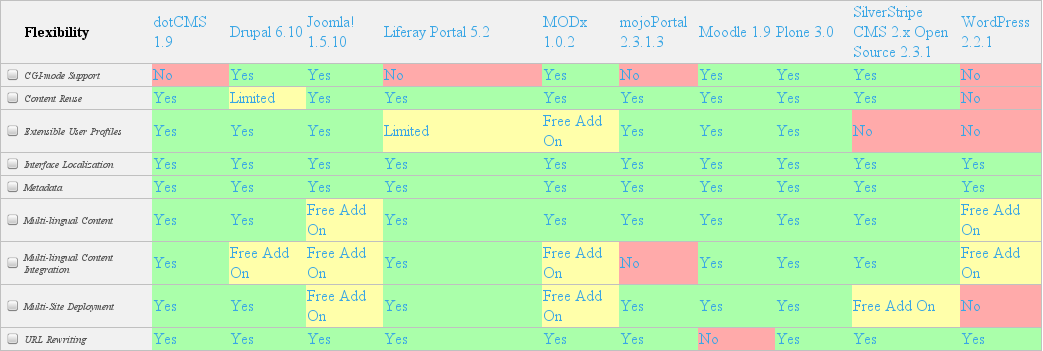
\includegraphics[width=\linewidth]{cmsmat8}
\caption{Flexibility desde CMSMatrix.org}
\end{narrow}
\label{fig:cmsmat8}
\end{figure}


\paragraph{Built-in Applications (Aplicaciones embebidas)}


\par En esta sección se presentan todas esas funcionalidades extras que podrían (o no) interesarnos a la hora de diseñar nuestra plataforma. 

\begin{figure}
\begin{narrow}{-0.12\linewidth}{-0.12\linewidth}
\centering
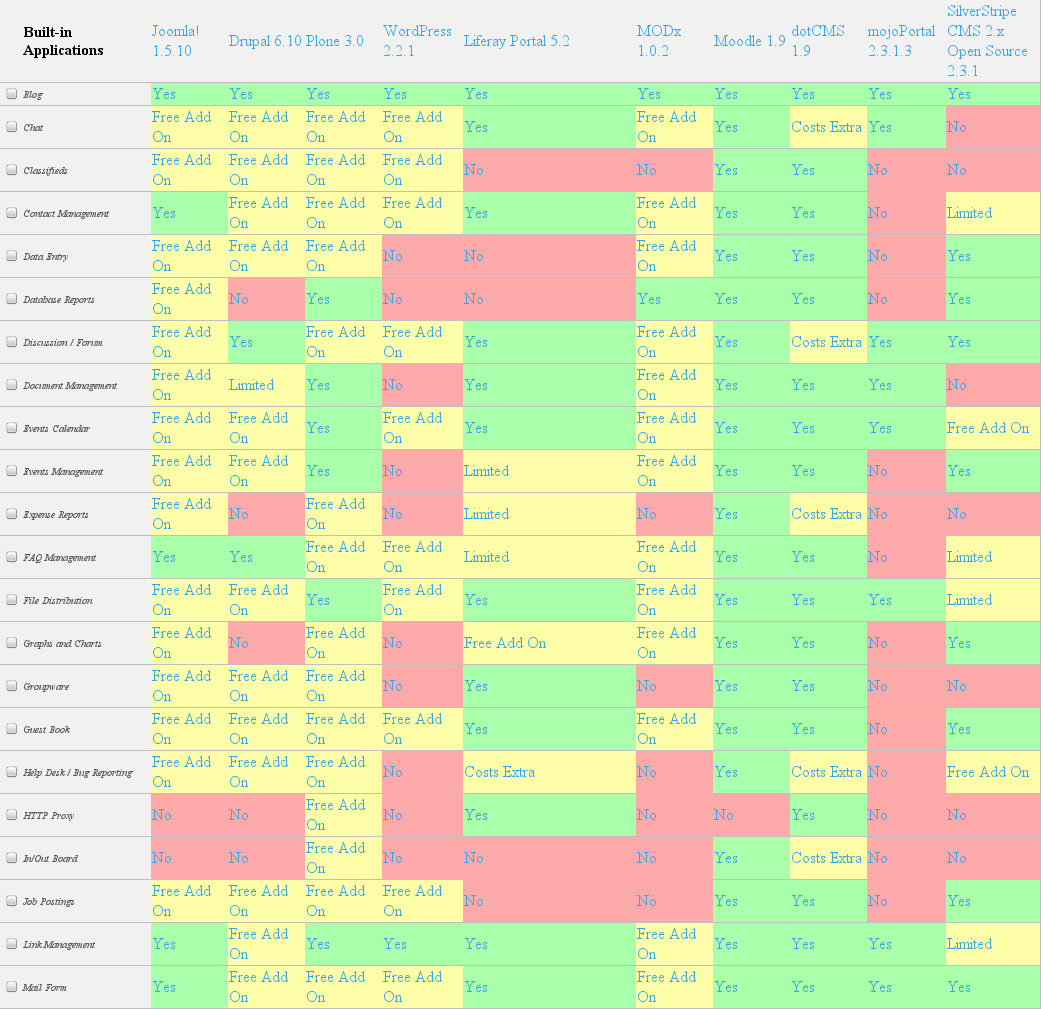
\includegraphics[width=\linewidth]{cmsmat9-1}
\caption{Built-in Applications (I) desde CMSMatrix.org}
\end{narrow}
\label{fig:cmsmat9}
\end{figure}

\par Entre las presentes, me parecen reseñables las que tienen que ver con calendarios y eventos, manejo de enlaces, encuestas, manejo de documentos y galería de imágenes, entre otras, aunque, en general, no son demasiado importantes porque no sería difícil recrearlas.

\begin{figure}
\begin{narrow}{-0.12\linewidth}{-0.12\linewidth}
\centering
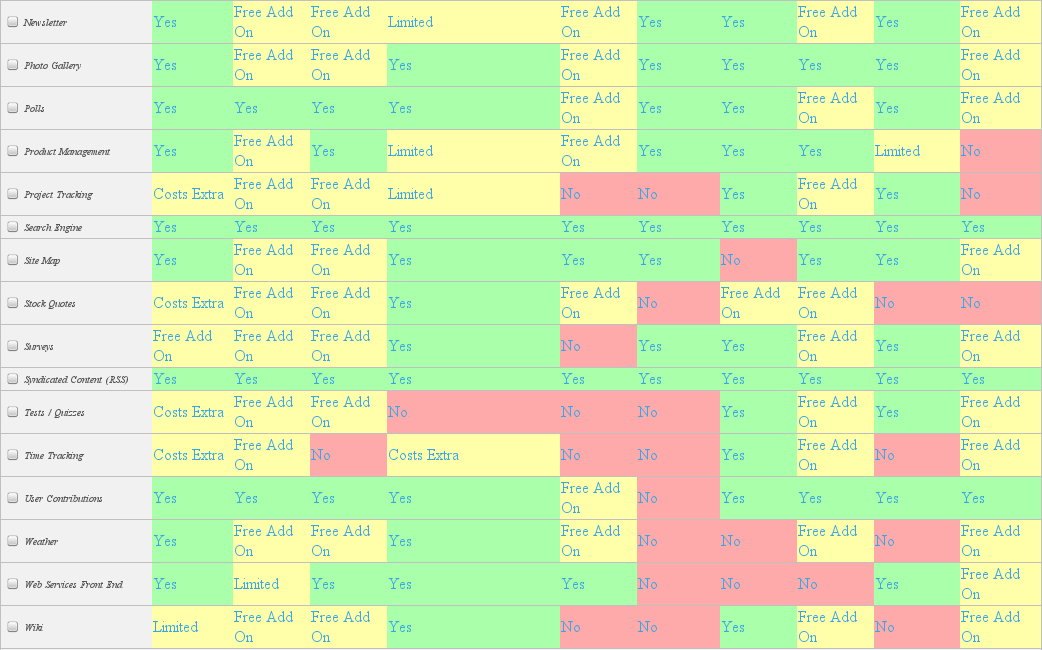
\includegraphics[width=\linewidth]{cmsmat9-2}
\caption{Built-in Applications (II) desde CMSMatrix.org}
\end{narrow}
\end{figure}

\paragraph{Commerce (Comercio electrónico)}


\par Esta última se incluye casi a modo testimonial, dado que la parte comercial tanto del museo como, más generalmente, de todo el IGN, se concentra en otro departamento, fuera del alcance de este proyecto. En ella podemos ver distintas funcionalidades orientadas a la parte más comercial de la actividad: tienda, carrito, pasarela, etc.

\begin{figure}
\begin{narrow}{-0.12\linewidth}{-0.12\linewidth}
\centering
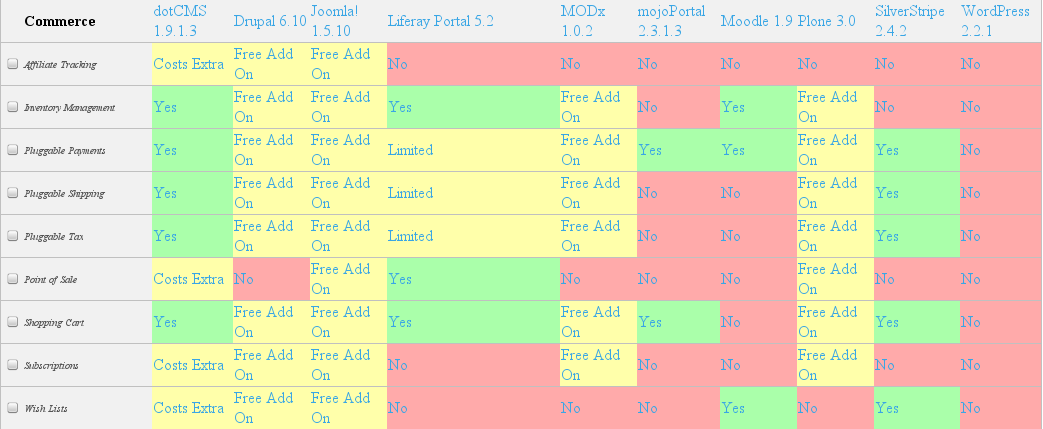
\includegraphics[width=\linewidth]{cmsmatA}
\caption{Commerce desde CMSMatrix.org}
\end{narrow}
\label{fig:cmsmatA}
\end{figure}



\par Dicho todo esto, considero que Joomla! también debería ser apartado de los candidatos dada la falla en cuanto a XHTML. Los costes extra de dotCMS para algunas características me hacen pensar que la filosofía de ese proyecto no es tan cercana a nuestros objetivos como podría parecer, así que también los desaconsejaría.


\subsubsection{Propuesta preliminar}
\par Los candidatos serán cuatro. Todos ellos son multiplataforma, corren en cualquier servidor y se componen de código abierto. Todos, además, disponen de interfaz en idioma español e inglés (como mínimo), galería de fotos y sistema de control de versiones (más o menos completo). Todos funcionan alimentándose de una base de datos con API estándar.
\par Como particularidades reseñables, podemos decir que, en cuanto a servidor web, Plone y Drupal están muy bien integrados con Apache, mientras que Liferay Portal se integra con otros servidores más orientados a Java (Tomcat, Glassfish, etc.) y Moodle que se integra con cualquier plataforma que tenga soporte para PHP.

\paragraph{Liferay Portal (Community Edition)}
\par Esta herramienta no presenta inconvenientes importantes ahora que su código es libre \cite{references:liferaylicense}, pues antes no era así. Más a su favor, tiene una empresa como IBM detrás lo que supone que su código viene siendo mantenido y desarrollado por profesionales. Es una solución seria, empresarial y con una curva de aprendizaje media. Se usa en sitios como los de CISCO, Honda, T-Mobile, Harvard Bussiness School, China Mobile, etc.
La rumorología parece indicar que sería la solución que el Instituto Geográfico Nacional estaría adoptando para su gestión de contenidos hipertextuales, con lo que, de ser cierto, ganaría puntos como solución definitiva, dado que habría personal cualificado para mantener la aplicación si fuese necesario.
Además de todo lo anterior, posee soporte comercial consolidado y está bastante probado.
\par Todo lo anterior la convierte en la opción más sólida a mi modo de ver.

\paragraph{Drupal}
\par Se trata de una de las plataformas más populares y amigables para la gestión de contenidos. Es usada para todo tipo de proyectos desde poco importantes hasta de envergadura media-alta. Sin embargo, no parece (por lo leído en algunos artículos) que sea la opción más potente.
No tiene, tampoco, carencias que señalar, destacando, eso sí, su carácter modular, necesitando así para algunas de las funcionalidades deseables de la instalación de módulos adicionales (gratuitos). Tiene una gran base de usuarios y está mantenido por la comunidad principalmente. Destaca, además, por su buena integración con plataformas móviles.
Es rápido, intuitivo y versátil.

\paragraph{Moodle}
\par Este CMS está orientado más al e-learning aunque es cierto que cumple con pŕacticamente todas las funciones deseables.
Se trata de un software maduro y completo.
Está programado en PHP, al igual que el anterior.

\paragraph{Plone}
\par Probablemente este CMS sea el más innovador de los presentados. Muy potente, está programado en Python y construído encima del framework Zope, independiéntemente del servidor que vaya a correr por debajo (que en general será Apache).
Al igual que el resto, no presenta deficiencias importantes, si bien, como Drupal, está pensado de manera modular, con añadidos para según qué funciones.
Si hay que poner una pega (y no es trivial), es su curva de aprendizaje, dado que llena los huecos dejados por Drupal en cuanto a potencia pero también en cuanto a dificultad de uso haciéndolo una opción no recomendable para no-informáticos, quizá.

\subsection{Anexo a comparativa}
\par Como resultado de la comunicación con el cliente, se hace una rápida referencia a una plataforma como candidata a ser la destinataria de la migración del CMS de todo el Instituto Geográfico Nacional. Normalmente, todo lo relacionado con la gestión de contenidos y, en general, todo el software generado suele ser subcontratado a otras empresas, dejando los desarrollos propios o artesanales casi exclusiva y paradójicamente al personal especializado (astrónomos, físicos, etc.).
\par La propuesta es analizar brevemente el candidato ``Alfresco'' para ver si sería viable tenerlo en cuenta como candidato para nuestro desarrollo.
\subsubsection{Breve análisis de Alfresco}
\par Para proceder con este análisis, la principal fuente de información será el sitio web de la compañía dedicado a hablar de la entidad. Alfresco es una empresa fundada por John Newton (Documentum\footnote{Empresa americana dedicada a la creación de un gestor de contenidos empresariales con el mismo nombre, hoy mantenido por EMC Corporation.\cite{references:documentum}}) y John Powell (Bussiness Objects\footnote{Empresa francesa dedicada a Bussiness Intelligence y desde 2007 parte de SAP AG\cite{references:bussinessobjects}}) e integrada por ingenieros de Documentum y Oracle en 2005 con capital de diferentes empresas de inversión como SAP Ventures, Accel Partners y Mayfield Fund. Se autodenominan la ``alternativa de código abierto para la gestión de contenidos empresariales (ECM)\cite{references:alfrescoabout}.
\par Aquí aparece un concepto desconocido hasta ahora en este documento: gestión de contenidos empresariales. Según la Asociación para la gestión de imágenes e información (AIIM en inglés), ECM se define como \cite{references:ecmaiim}: ``las estrategias, métodos y herramientas usadas para capturar, gestionar, almacenar, preservar y entregar contenido y documentos relacionados con procesos organizativos. Las estrategias y herramientas ECM permiten la administración de la información no estructurada de una organización donde quiera que ésta exista."\renewcommand{\thefootnote}{\fnsymbol{footnote}}\footnote[1]{Traducción propia.}\renewcommand{\thefootnote}{\arabic{footnote}}	

\par Aunque quizá ya era de esperar, podemos ver que este tipo de plataforma abarca mucho más de lo que en principio necesitaríamos y está enfocado de manera diferente a lo que sería nuestro museo virtual. Si nos atenemos a la plataforma, rápidamente vemos que forma parte del modelo de negocio que algunas empreas han encontrado para explotar el código abierto: el soporte. No hay otra manera (salvo una evaluación de 30 días) de utilizar la plataforma Enterprise que la de contratar una suscripción con la empresa atendiendo a diversos paquetes de soporte integrado. Las características incluídas en todas las opciones son:

\begin{itemize}
\item Pruebas certificadas de escabilidad
\item Un modelo controlado del lanzamiento
\item Mantenimiento y Actualizaciones
\item Resolución de Problemas
\item Consejos de Configuración, Compatibilidad y Migraciones
\item Soporte de Actualización
\item Consejos de Puesta a punto
\item Tiempos de reacción garantizados
\end{itemize}

\par Como todo sitio corporativo, su lenguaje es marcadamente general por lo que conviene entrar un poco más en detalle. Para ello podemos utilizar el mismo recurso antes mencionado de CMSMatrix.org\cite{refrences:alfrescocmsmat}. En este caso, no tenemos muy clara cuál es la plataforma analizada, ya que Alfresco se presenta en distintos sabores\cite{references:alfrescocomp}: Cloud Trial (prueba online, no incluye gestión de contenidos web, Alfresco Enterprise (probada y certificada para plataformas tanto código abierto como propietarias, con soporte comercial completo) y Alfresco Community (para plataformas de código abierto, soportada por la comunidad).

\par Debido a la variabilidad de plazos y la diferencia apreciable de alcance en los proyectos del IGN y de este proyecto respectivamente, al final se decidió abandonar la línea de Alfresco sobre Liferay Portal y se optó por Drupal, que reunía los requisitos adecuados y tiene una gran comunidad de usuarios y desarrolladores detrás.

Sin embargo, he creído conveniente adjuntar un anexo donde se indague un poco más sobre Alfresco y sus posibilidades.

\subsection{Modelo de datos}
\par Hemos dejado bien claro que el propósito de este trabajo no es desarrollar de cero un CMS si no escoger y adaptar uno ya existente a las necesidades que se nos han presentado. Antes de tomar una decisión (que es independiente del autor y tomará tiempo), es conveniente señalar que sí que debería existir una parte de ``diseño original'' que correspondería al modelado de algunas informaciones. 


\subsubsection{Catálogo}
\par Respondiendo a los requisitos enunciados por miembros de la empresa, he elaborado un diseño de modelo de datos que podría utilizarse para abstraer los contenidos de un catálogo de objetos expuestos (subconjunto de ítems informativos del total del museo virtual) y no expuestos.
Para ello, me he ayudado de un catálogo editado en papel por el propio Ministerio de Fomento titulado ``Instrumentos históricos del Instituto Geográfico Nacional". Debido a su creación artesanal cada instrumento no sigue la debida canonización que nos piden las bases de datos, y es por eso que he tratado de ordenarlo en un modelo de datos como el que se muestra:

\paragraph{OBJETO}
\begin{itemize}
\item id/ref: número entero
\item nombre: caracteres(30)
\item firmado: (inventor, lugar\_origen, fecha\_origen) (se eliminaría del original)
\item inventor: relación(n:n)
\item lugar\_origen: relación(n:n)
\item fecha\_origen: fecha
\item dimensiones: caracteres(12)
\item características técnicas: texto
\item materiales: caracteres(20)
\item depósito\_habitual: relación(1:n)
\item observaciones: texto
\item área: relación(1:1)
\item tipo de objeto: relación(1:n)
\item foto: caracteres(50)
\item depósito actual: caracteres(50)
\end{itemize}

\paragraph{ÁREA}
\begin{itemize}
\item id: numerico
\item nom\_area: caracteres(20)
{Astronomía esférica, Geodesia geométrica, Topografía planisférica y Fotogrametría terrestre.
Topografía altimétrica, Gabinete, Meteorología, Geofísica}
\end{itemize}

\paragraph{TIPO\_OBJETO}
\begin{itemize}
\item id: numerico
\item nom\_tipo: caracteres(40)
\item id\_area: relacion(n:1)
\end{itemize}

\paragraph{ARTÍCULOS}
\begin{itemize}
\item id: numerico
\item titulo: caracteres(25)
\item contenido: texto
\end{itemize}

\paragraph{AREA\_ARTÍCULO}
\begin{itemize}
\item id\_area: relación(1:n)
\item id\_articulo: relacion(n:1)
\end{itemize}

\paragraph{INVENTOR}
\begin{itemize}
\item id\_inventor: numerico
\item nom\_inventor: caracteres(25)
\end{itemize}

\par Este modelo será reutilizado (si se aprueba) para crear una interfaz sencilla de entrada de datos para el personal interno.
%  \centering
%   \includegraphics[width=\textheight]{proyecto2}
%\caption{Diagrama de Gantt del proyecto}
%\label{fig:gantt2}
%\end{sidewaysfigure}

\section{Drupal}

\par Como dije más arriba, Drupal será incialmente la plataforma seleccionada para comenzar con la integración y desarrollo del sistema. Se trata de un sistema complejo, del que prefiero describir algunos fundamentos básicos que ayunden a entenderlo todo.

\par Existen multitud de recursos en Internet sobre Drupal, empezando por su sitio web principal \cite{references:drupalhome}, pero el recurso más útil que he encontrado es el libro editado por O'Reilly \cite{ByronBerryHaugEatonWalkerRobbins200812} y creado por el staff del sitio web Lullabot \cite{references:lullabot}. Aunque la versión traducida al español editada por Anaya \cite{ByronBerryHaugEatonWalkerRobbins200909} facilita el seguimiento general del libro, considero que en algunos aspectos es una traducción, cuanto menos, apresurada.

\subsection{Entorno de (pre)desarrollo}
\par Para la prueba inicial he utilizado un ``software appliance", es decir, una imagen de disco dispuesta a ser arrancada por una máquina virtual (en este caso VirtualBox) y empezar a funcionar. esto facilita mucho las cosas a la hora de realizar configuraciones rápidas y dinámicas dejando para más adelante (cuando tengamos una arquitectura definida) la integración y configuración de un servidor real.

La máquina elegida fue sacada de la web de TurnKey \cite{references:turnkey} en la que se pueden encontrar multitud de imágenes listas para hacer la función de servidor web con CMS nada más ser arrancadas. Suele tratarse de un montaje LAMP (Linux + Apache + MySQL + PHP) \cite{references:LAMP} En concreto se utilizó la que integraba la versión 6 de Drupal \cite{references:turnkeydrupal} con un entorno que se describe con los siguientes componentes básicos:

\begin{itemize}
\item TurnKey Core \cite{references:turnkeycore}, compuesto de:
	\begin{itemize}
	\item Ubuntu 8.04.3 LTS
	\item Autoactualizable en el arranque
	\item Shell en AJAX incorporada (shellinabox\cite{references:shellinabox})
	\item Interfaz de administración web (Webmin\cite{references:webmin})
	\item Apache, MySQL y PHP.
	\end{itemize}
\item Soporte para SSH por defecto.
\item MTA integrado para el envío de correo local.
\item Módulos de Webmin para PHP, Apache2 y MySQL.
\item PHPMyAdmin como administrador de la base de datos.
\item Módulos más conocidos de Drupal (CCK, Views, Lightbox2, ImageCache, CKEditor, etc.).
\end{itemize}

\par En este caso, a la configuración inicial se le hicieron varias modificaciones, como instalar la distribución en español (que era uno de los requisitos) e instalar un módulo FTP en Webmin. Para la primera cosa hubo que borrar la instalación que venía por defecto con el ``appliance'' y volver a instalar Drupal en español descargándolo desde su página\cite{references:drupalhispano}. Para la segunda, sin embargo, salvo modificar ligeramente permisos en el servidor via SSH, el propio Webmin es bastante intuitivo.

\subsection{Understanding Drupal}

\par Como en el libro original, una buena manera de comenzar nuestro periplo por este CMS es conocer sus fundamentos.
\par Se vió más arriba que Drupal es un CMS gratuito y de código abierto con una amplia comunidad de usuarios y colaboradores, lo que lo convierte en una plataforma bastante actualizada, potente y en contacto con las necesidades demandadas por la mayoría de usuarios.

\subsubsection{General} 

\par En su concepción, Drupal no necesita un sistema operativo, servidor web o gestor de bases de datos concreto. Puede valer cualquiera capaz de correr una implementación de PHP y una base de datos compatible con SQL. Digamos que el ``alma'' de Drupal estaría contenida en la base de datos y se articularía gracias al ``core'' que hace uso del intérprete PHP. Además de los subsistemas que permiten el interpretado de temas gráficos, la gestión de sesiones de usuario y el filtrado para mantener la seguridad del sistema. Alrededor de este núcleo tendríamos los módulos (tanto incluídos por defecto como los que han sido asimilados gracias a la comunidad de desarrolladores) que extenderían la funcionalidad del sistema a lugares más específicos que van desde la creación de contenidos hasta la asistencia a tareas de administración pasando por todo tipo de funciones imaginables.
Los contenidos de Drupal se basan en un concepto simple pero efectivo: los nodos. Todos los contenidos son organizados en nodos que pueden ser accedidos independientemente. Serían, por así decirlo, las unidades mínimas de contenido en Drupal. Todos ellos, además de los temas, configuraciones y usuarios se almacenan en la base de datos. A la hora de servir las páginas, el motor de Drupal en PHP trasladará esa información de la base de datos, produciendo una salida en XHTML con CSS (al menos, predeterminadamente) gracias a la interpretación de las plantillas que acompañan a los temas gráficos.

\subsubsection{Módulos} 

\par Los módulos, tanto los que se incluyen oficialmente junto al ``core", como los que son aportados y mantenidos por la comunidad desarrolladores, son los que aportan la funcionalidad más cercana al usuario. Articulan lo que de otra manera sería una simple plataforma de edición de páginas web con una base de datos como soporte fundamental.
En esencia, son archivos que contienen código php que proporciona un conjunto de funcionalidades y se integran en Drupal. Estas funcionalidades, salvo en las excepciones de módulos necesarios para el funcionamiento ``nuclear'' de Drupal, pueden ser activados o desactivados en cualquier momento, claro está, atendiendo a las interdependencias entre unos módulos y otros.
\par Prácticamente todas las funcionalidades, desde la gestión de usuarios y credenciales (módulo User) o los formularios de contacto con el responsable de la página (módulo Contact) hasta la creación de Galerías de imágenes o taxónomías para ordenar el contenido semánticamente, son aportadas por estos componentes.
La verdadera potencia de los módulos reside en la interconexión de los mismos y el ajuste minucioso de las numerosas opciones de configuración que aporta cada uno de ellos. Nunca podrá conseguirse un sistema a pleno rendimiento si las opciones se dejan por defecto (aunque esta generalidad aplica a todo sistema informático de cierto nivel). Esta potencia que se nos ofrece en un principio, puede, dado la gran cantidad de alternativas disponibles, sin embargo, convertirse en un dolor de cabeza para dar con el módulo adecuado a nuestras necesidades (dado que hay varios que pueden aportar similares funcionalidades).

\subsubsection{Usuarios} 

\par Una de los cuerpos más importantes de un sistema informático es la gestión de usuarios. Su mayor baza es la de personalizar el entorno según las credenciales de la persona (o máquina) que accede. En el caso de Drupal, por defecto, encontramos un sistema de usuarios con multitud de opciones. Por defecto, se crea el ``User 1", que sería algo así como el usuario ``root'' en sistemas UNIX, es decir, un superusuario con derechos plenos sobre todo el sistema.
Si bien la clásica organización en usuarios podría ser una solución, en el caso de Drupal, se añade el concepto de ``rol. Un rol, siguiendo con la analogía de UNIX, sería algo similar a un grupo de usuarios. De esta manera, se permite separar el espacio individual posible de cada usuario (que en nuestro caso no tendría demasiada utilidad, salvo la meramente identificativa a la hora de hacer cambios y puede que la capacidad de tener entradas como borradores) de su asignación de permisos.
Los permisos son asignados a un rol determinado, y ese rol determinado puede ser asignado a varios usuarios, permitiendo, en todo caso, que todo usuario (incluso los anónimos) estén bajo control a la hora de decidir el acceso, creación, modificación y borrado de datos, así como los contenidos presentados en cada caso.

\subsubsection{Nodos} 

\par Este punto podría decirse que es la piedra angular de Drupal. Si en un CMS lo importante son los contenidos, en Drupal, si queremos hablar de contenidos, tenemos que remitirnos a los nodos. Como dijimos anteriormente, los nodos son la unidad mínima de publicación de contenidos en Drupal. No es raro, al visitar un sitio al azar (dada la extendida implantación de Drupal en los sitios web) que topemos con urls que contengan, entre barras, la palabra ``node", aunque esto sea, según algunos gurús, algo a evitar por los desarrolladores, ya sea mediante alias que escondan esas urls o mediante plantillas que engloben los nodos como un componente más.
Y ahí radica una de las característica más poderosas de los nodos y es que pueden ser tomados como partes de estructuras más grandes, permitiendo cosas como que una foto, su título, y si se quiere, un comentario, puedan ser en sí mismas un nodo, y a su vez, este nodo, formar parte como referencia en otro nodo. 
Todo esto aporta una fortaleza importante a la hora de indexar contenidos, proyectar búsquedas o presentar las entradas de diferentes maneras y atendiendo a unos y otros criterios, ya que todos los contenidos parten de una estructura común y son, hasta cierto punto, compatibles entre sí.

\par Los nodos, en su estructura más básica, están compuestos por:
\begin{itemize}
\item Autor
\item Fecha de creación
\item Título del nodo
\item Contenido principal
\end{itemize}

\par A partir de ahí pueden darse diferenciaciones o mutaciones que permitan distinguir entre distintos tipos de contenido. Como por ejemplo la diferencia existente entre Página (Page) y Artículo (Story), que prepara la página para ser un contenido esencialmente estático e informativo (incluso institucional) y el artículo para ser algo más dinámico, corriente y genérico. ``Page'' y ``Story'' son los dos medios básicos que son incluidos por defecto en Drupal, dejando Page para páginas tipo ``¿Quiénes somos?'' o ``Política de privacidad", que no requieren interactividad, ni cambios y que están preparadas para ocultar por defecto la fecha y el autor del contenido. Sin embargo, ``Story'' contaría con la intención (al menos en su creación) de formar parte de lo que llamaríamos la portada del sitio, como una ``noticia'' más o una ``novedad'' más, que tiene un contexto temporal y un autor más relevantes.

\par Combinando las dos funcionalidades pasasdas podremos asignar las capacidades de los usuarios (a través de sus roles asignados) individualmente para cada tipo de contenido. Dejando, puede ser, un contenido institucional a un editor y un contenido más dinámico a un redactor (o cualquier otra combinación que se nos ocurra).

\subsubsection{Formas de organizar el contenido}

\par Dejando de lado la parte más semántica e íntegra del sistema, las cuestiones organizativas son las que afloran. En este caso, hay distintas aproximaciones posibles que nos permiten presentar y complementar los contenidos descritos más arriba.

\paragraph{Bloques}

\par Pasando a la parte más visible (la v dentro del modelo MVC) aunque con ramificaciones en las otras dos, nos encontramos con esta estructura. Los bloques constituyen las unidades más pequeñas para mostrar información. Digamos que son pequeños trozos de código que aportan una funcionalidad que se plasmará visiblemente en la pantalla. Cosas como el número de usuarios conectados, los últimos comentarios en entradas o los artículos más populares son los ejemplos más conocidos de este tipo de objetos, que seguro que son conocidas a la mayoría de usuarios medios por haber visto cosas similares en otros sitios de la red.

\par Se enmarcan en regiones distribuidas por la estructura gráfica de la página (como encabezado, pie, laterales o cuerpo principal). Serían, pues, los diferentes componentes que podríamos organizar (o quitar) de nuestra página para que mostrase la información que consideramos necesaria. Juegan un papel fundamental a la hora de trabajar con plantillas, que veremos en el apartado de Temas.


\paragraph{Menús}

\par No hay mucho que explicar sobre los menús en Drupal salvo que son, como casi todo, altamente personalizables. Serían colecciones de enlaces que normalmente están situados en regiones reconocibles de nuestro sitio web y nos permiten movernos por el sitio sin perdernos y sin dar muchos rodeos. Dependiendo de cómo están construidos pueden incluso darnos una idea de dónde estamos. Por defecto se crea un menú principal que se mostraría en todo momento y un secundario que se mostraría a partir de la opción seleccionada en el menú principal. Su uso, como desde hace mucho tiempo, es muy intuitivo.

\paragraph{Taxonomías}

\par Aunque hablaremos más adelante de esto, hay que reseñar que el módulo ``Taxonomy'' nos proporciona una funcionalidad que en nuestro caso vendrá a sustituir por ahora lo que en principio se iba a construir a base de ontologías y redes semánticas. Es una implementación muy simple pero en nuestro caso resulta que cumple con nuestras necesidades. Permitiría clasificar los contenidos (incluso haciendo distinciones entre distintos tipos de contenido) según clasificaciones que nosotros previamente hayamos creado, a las que el programa llamará ``vocabularios". Es decir, que en función de la clasificación (o clasificaciones, dado que se pueden aplicar varias a la vez) que le otorguemos a un contenido en concreto, podrá ser posteriormente relacionado en una jerarquía que ordenará los contenidos por su área semántica. Por inmediatez del ejemplo, podremos catalogar los instrumentos de nuestro museo por área de conocimiento a la que pertenecen (astronomía, geofísica, geodesia, ...) y a la vez enmarcarlos en una época temporal, por los materiales de su construcción (pudiendo estar a la vez en varios grupos) o por cualquier otra escala que se nos ocurra.
\par Esta funcionalidad, combinada con la anterior de los menús, puede ser muy interesante a la hora de ayudar al usuario a navegar con sentido por el sistema.

\paragraph{CCK (Content Construction Kit)}
\par Si uno de los puntos fuertes de Drupal es la definición de tipos de contenido a través del concepto de ``nodo'', el Kit de consturcción de contenido (CCK) nos permite estructurar semántica y lógicamente cada uno de los apartados de nuestro tipo de contenido. En definitiva, proporciona una herramienta para especificar campos concretos (con su definición de tipo de datos) que contengan datos definidos, como en el caso de un registro, que contiene campos. En este caso, podremos elegir el nombre de la variable o campo, el tipo de datos que contendrá y, en su caso, qué interfaz (o widget) se le presentará al usuario a la hora de tener que rellenar ese campo. Es un módulo tan esencial que a partir de la versión 7 de Drupal forma parte del núcleo de la plataforma. Digamos que es un paso más hacia la ingeniería de software más clásica.

\paragraph{Views}
\par El módulo anterior se complementa a la perfección con otro módulo más: se trata de Views, y como su propio nombre indica, su cometido es asistir a la hora de la creación de vistas personalizadas. Aludiendo estas a muy diversos parámetros que regulan desde quién verá cada vista, pasando por los campos que se mostrarán de cada nodo, parámetros disponibles para realizar búsquedas o la manera que tendremos de mostrar el contenido al usuario.
\par Se trata de un módulo muy potente y, para hacerse una idea, recoge cierto paralelismo con las ``vistas'' de una base de datos SQL. De hecho, se puede, incluso, proporcionar código SQL que defina (con la potencia que eso implica) en detalle la consulta que queremos hacer a la hora de ejecutar una vista.

\subsubsection{Temas}
\par Los temas son la cara visible de Drupal hacia el usuario, son un conjunto de ficheros CSS, HTML/PHP e imágenes que permiten dar forma a la salida por defecto del contenido. Sería lo correspondiente a la capa de visualización o a la parte de vista en el modelo MVC. La noción de ``tema'' se supone conocida en este ámbito. Brevemente, el paso de una url a html supondría dar los pasos de:
\begin{enumerate}
\item El módulo Node recibe la petición (http://www.dominio.com/node/2)
\item Node extrae el contenido del nodo y llama al módulo Theme
\item Theme, a través del motor del tema, estructura el contenido de la salida
\item Se le aplica el aspecto gráfico del tema utilizado en ese momento.
\end{enumerate}

\par Sin embargo, se podría ilustrar la estructura usada por Drupal a través de un pequeño esquema \cite{fig:drupalthemes1}
\begin{figure}
\begin{narrow}{-0.12\linewidth}{-0.12\linewidth}
\centering
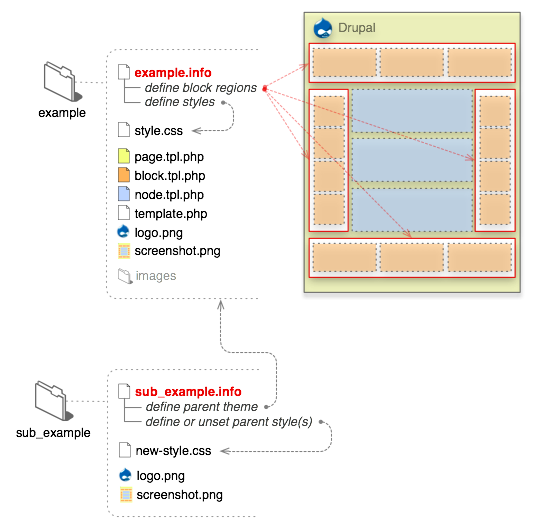
\includegraphics[width=\linewidth]{drupalthemes1}
\caption{Estructura básica de Temas en Drupal\cite{references:drupalthemes}}
\end{narrow}
\label{fig:drupalthemes1}
\end{figure}

 
\paragraph{Archivos .info}
\par Este tipo de archivos, ubicados normalmente en la carpeta ``themes'', define, obligatoriamente, metadatos del tema en concreto como su nombre, descripción, versiones de Drupal con las que es compatible y el motor de temas que usa. Igualmente, puede incluir la definición de regiones en las que dividiremos nuestro tema, los ficheros CSS y/o JavaScript que lo acompañarán o las funcionalidades que el administrador podrá utilizar en el panel de administración de temas.

\paragraph{Regiones}
\par Se trata de las divisiones del espacio gráfico que definirá nuestro tema y en las que se pueden ubicar los bloques. Las definidas por defecto en Drupal son:
\begin{itemize}
\item Header (encabezamiento)
\item Footer (pie de página)
\item Left Sidebar (bara lateral izquierda)
\item Right Sidebar (barra lateral derecha)
\item Content (sección central dedicada al contenido)
\end{itemize}

\par Por supuesto, como todo en Drupal, podemos definir las nuestras propias. Eso sí, en el momento en que creemos nuestro propio fichero .info y definamos una sola región, las regiones por defecto no serán tenidas en cuenta si no se refieren explícitamente.

\paragraph{Características}
\par Se trata de todas esas opciones que podrán ser administradas desde el panel de administración de Drupal. Entre ellas encontramos, por defecto, las siguientes:

\begin{itemize}
\item Logotipo (logo)
\item Nombre del sitio (name)
\item Lema (o eslogan) del sitio (slogan)
\item Declaración de intenciones (mission)
\item Avatar de usuario en entradas (node_user_picture)
\item Avatar de usuario en comentarios (comment_user_picture)
\item Cuadro de búsqueda (search)
\item Icono del navegador / marcadores (favicon)
\item Enlaces primarios del menú (primary_links)
\item Enlaces secundarios del menú (secondary_links)
\end{itemize}

\par De la misma manera que ocurría con las regiones, las características también son personalizables aquí.

\paragraph{CSS y JavaScript}
\par Como en las otras ocasiones, existen algunas rutas por defecto para incluir nuestro código CSS y JavaScript en nuestro proyecto, pero además podemos redefinir y añadir las referencias de nuestros ficheros adicionales.

\paragraph{Archivos de plantilla}
\par Aquí es donde reside la mayoría de la maquetación real de las páginas. Estos archivos, con abundancia de código HTML y algunas sentencias PHP desvelan la estructura que presentarán a la salida cada uno de los elementos de contenido. La extensión de los archivos es del tipo <elemento>.tpl.php, como por ejemplo page.tpl.php o node.tpl.php. Dentro de ellos, las sentencias de php interrogan a la base de datos para saber si se han completado las regiones correspondientes para rellenarlas de contenido y darles una forma.

\paragraph{template.php}
\par Esta sería la piedra angular de todo programador, ya que se utiliza para añadir lógica y variables a la aplicación y para redefinir funciones que son llamadas por los archivos de plantilla. Se trata, casi exclusivamente, de código php por lo que deberían ser editados por programadores o diseñadores con conocimientos de este lenguaje.




\section{Conclusiones y trabajo futuro}



\clearemptydoublepage

\chapter{Planos}
\newpage
\clearemptydoublepage
\section{Esquemáticos}
Aqu tenemos los esquemticos.
\clearemptydoublepage

\chapter{Pliego de condiciones}
\newpage
\clearemptydoublepage
\section{Requisitos de Hardware}
Estos son los requisitos mnimos de Hardware
\section{Requisitos de Software}
Estos son los requisitos mnimos de Software
\clearemptydoublepage

\chapter{Presupuesto}
\newpage
\clearemptydoublepage
\section{Presupuesto}
En esta seccin se detalla el presupuesto de ejecucin del proyecto.

\clearemptydoublepage

\chapter{Manual de Usuario}
\newpage
\clearemptydoublepage
\section{Manual}
En esta sección se resumirá el manual de usuario de la aplicación en cada caso.


\clearemptydoublepage

\chapter{Soporte informático}
\newpage
\clearemptydoublepage
\include{soporte}
\clearemptydoublepage

%\chapter{Apéndices}
%\newpage
%\clearemptydoublepage
%\section{Apéndice I: Alfresco}
\label{cha:apendicealfresco}
\par La propuesta es analizar brevemente el candidato ``Alfresco'' para ver si sería viable tenerlo en cuenta como candidato para nuestro desarrollo.

\subsection{Análisis}
\par Para proceder con este análisis, la principal fuente de información será el sitio web de la compañía dedicado a hablar de la entidad. Alfresco es una empresa fundada por John Newton (Documentum\footnote{Empresa americana dedicada a la creación de un gestor de contenidos empresariales con el mismo nombre, hoy mantenido por EMC Corporation.\cite{references:documentum}}) y John Powell (Bussiness Objects\footnote{Empresa francesa dedicada a Bussiness Intelligence y desde 2007 parte de SAP AG\cite{references:bussinessobjects}}) e integrada por ingenieros de Documentum y Oracle en 2005 con capital de diferentes empresas de inversión como SAP Ventures, Accel Partners y Mayfield Fund. Se autodenominan la ``alternativa de código abierto para la gestión de contenidos empresariales (ECM)\cite{references:alfrescoabout}.
\par Aquí aparece un concepto desconocido hasta ahora en este documento: gestión de contenidos empresariales. Según la Asociación para la gestión de imágenes e información (AIIM en inglés), ECM se define como \cite{references:ecmaiim}: ``las estrategias, métodos y herramientas usadas para capturar, gestionar, almacenar, preservar y entregar contenido y documentos relacionados con procesos organizativos. Las estrategias y herramientas ECM permiten la administración de la información no estructurada de una organización donde quiera que ésta exista."\renewcommand{\thefootnote}{\fnsymbol{footnote}}\footnote[1]{Traducción propia.}\renewcommand{\thefootnote}{\arabic{footnote}}

\subsubsection{Sabores}
\par Aunque quizá ya era de esperar, podemos ver que este tipo de plataforma abarca mucho más de lo que en principio necesitaríamos y está enfocado de manera diferente a lo que sería nuestro museo virtual. Si nos atenemos a la plataforma, rápidamente vemos que forma parte del modelo de negocio que algunas empresa han encontrado para explotar el código abierto: el soporte. No hay otra manera (salvo una evaluación de 30 días) de utilizar la plataforma Enterprise que la de contratar una suscripción con la empresa atendiendo a diversos paquetes de soporte integrado. Las características incluidas en todas las opciones son:

\begin{itemize}
\item Pruebas certificadas de escalabilidad
\item Un modelo controlado del lanzamiento
\item Mantenimiento y Actualizaciones
\item Resolución de Problemas
\item Consejos de Configuración, Compatibilidad y Migraciones
\item Soporte de Actualización
\item Consejos de Puesta a punto
\item Tiempos de reacción garantizados
\end{itemize}

\par Como todo sitio corporativo, su lenguaje es marcadamente general por lo que conviene entrar un poco más en detalle. Para ello podemos utilizar el mismo recurso antes mencionado de CMSMatrix.org\cite{references:cmsmatrix}. En este caso, no tenemos muy clara cuál es la plataforma analizada, ya que Alfresco se presenta en distintos sabores\cite{references:alfrescocomp}: Cloud Trial (prueba online, no incluye gestión de contenidos web, Alfresco Enterprise (probada y certificada para plataformas tanto código abierto como propietarias, con soporte comercial completo) y Alfresco Community (para plataformas de código abierto, soportada por la comunidad).

\par Desgraciadamente, la página de CMSMatrix.org muestra unos valores de comienzos del 2008 con lo que vamos a evitarnos el trabajo de listarla.


\subsubsection{Edición Web}

\par Alfresco se presenta como una opción flexible para desarrolladores. Para ello, ofrecen algo llamado Alfresco Quick Start. Se trata de una especie de sitio dinámico prefabricado construido en Spring Surf pero con el repositorio de contenidos marca de la casa (Alfresco Share). De hecho, lo mencionan en varios documentos como algo especial. Es traído a colación a cuento de que, al parecer, llega un momento en todo desarrollo de sitios dinámicos en el que el usuario acaba por pedir más y más control, lo que carga al desarrollador de un montón de trabajo tratando de implementar funciones sencillas de administración del sitio. Esta herramienta presume de traer todas esas características de fábrica, para permitir a los constructores de sitios web seguir con tareas más importantes como la experiencia de usuario final. En teoría, lo engorroso de la gestión de contenidos queda del lado de Alfresco Share.

\paragraph{Sitios colaborativos} 
\par Esta plataforma trata de simplificar, como toda aplicación informática presume, las tareas del usuario, dejando el horizonte libre para lo que sería, directamente, crear.
\par Entre otras características, cuenta con:
\begin{itemize}
 \item Edición Web en el navegador, lo que facilita mucho esta tarea al usuario final pudiendo valerse de contenidos previamente publicados.
 \item Integración de documentos ofimáticos automáticamente en la web (Office-to-Web), lo que permitiría, basándose en Google Docs (el sistema en la nube de edición colaborativa de documentos), con muy poco esfuerzo, pasar de bocetos en MS Office a publicar en la web respetando las normas CSS de la empresa.
 \item Unidad de red compartida, que no es más que extender el concepto que popularizó Microsoft hace muchos años pero en este caso, como si se tratase de la librería de la web.
\end{itemize}


\subsubsection{Gestión}
\par Alfresco propone, como adelantábamos, una gestión simplificada a base de herramientas ya creadas para facilitar las tareas más tediosas de la creación de sitios web. Defienden, además, que su plataforma no se acaba donde otros pretenden, en interfaces como la que podría proporcional Drupal o Webmin para gestionar un servidor, si no que, entre otras, destacan estas características:

\paragraph{Creación de nuevos sitos} Aunque esta no es la más novedosa de las opciones (pues podemos encontrar cosas similares en otras plataformas) sirve para fácilmente, a base de asistentes, crear nuevos sitios en el mismo entorno, incluso, compartiendo contenidos.

\paragraph{Modificación de la navegación} Podemos cambiar los flujos de información sin tener que modificar la estructura interna del sistema ni editar ficheros de configuración.

\paragraph{Definición de colecciones de contenido dinámico} Aunque esto tampoco es algo nuevo (Drupal, mismamente, lo incluye) constituye la habilidad para incluir, en esencia, módulos que se actualizan en el acto y, que, de hecho, muestran datos que se ven afectados por los pequeños eventos (últimas visitas, últimos comentarios, noticias mejor valoradas, etc.).

\subsubsection{Licencia y fundamentos}
\par Finalmente, sólo reseñar que Alfresco está construido enteramente sobre software libre y estándares abiertos y está distribuido bajo licencia Apache.
Se trata de una plataforma que proporciona herramientas muy optimizadas para permitir, sin esfuerzo, crear aplicaciones Web orientadas a los contenidos y basadas, en general en Java.

\subsection{Conclusiones}
\par Tras contemplar diversos artículos y white papers, parece ser que Alfresco está muy bien considerado por la crítica de CMS (que existe). Viene a ser llamado como la alternativa a Microsoft SharePoint, pudiendo competir con éste en el lado del software libre.
\par Respecto a lo que tiene que ver con este proyecto, y si bien es cierto que puede ser conveniente para organizaciones grandes como un ministerio o una dirección general para publicar sus contenidos entre otras cosas, por su sencillez y facilidad para trasladar los contenidos desde las fuentes más comunes (programas de ofimática) y por su muy bien pensado repositorio de contenidos de todo tipo (una especie de Evernote a lo grande y compartido), no corresponde con los intereses que acompañan a un museo virtual. El nuestro, pues, considero que es un sistema mucho más sencillo y desde luego más pequeño, en el que la colaboración propuesta por Alfresco sería casi más un obstáculo que una ventaja.

\par Por todo ello y por sus ofertas comerciales más orientadas a atraer clientes en el mundo empresarial, considero que no es el mejor candidato para el proyecto.
%\clearemptydoublepage

\chapter{Bibliografía}
\newpage
\clearemptydoublepage
% can use a bibliography generated by BibTeX as a .bbl file
% standard IEEE bibliography style from:
% http://www.ctan.org/tex-archive/macros/latex/contrib/supported/IEEEtran/bibtex

\bibliographystyle{./IEEEtran}
% argument is your BibTeX string definitions and bibliography database(s)
\bibliography{./IEEEabrv,./references}

%\bibliographystyle{unsrt}
%\bibliography{bibliografia}
\clearemptydoublepage

\printindex

\end{document}
